\documentclass{standalone}
\usepackage{tikz, tikz-cd}
\usetikzlibrary{shapes, decorations.markings}
\begin{document}

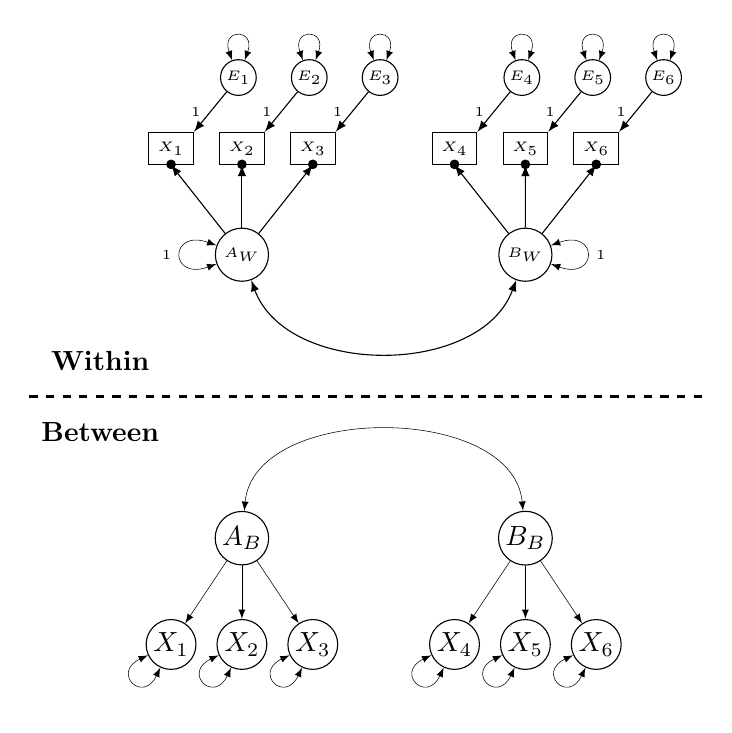
\begin{tikzpicture}[scale=0.9]
\node[draw, circle, inner sep=2] (l1) at (2,2) {\tiny{$A_W$}};
\node[draw] (o1) at (1,3.5) {\tiny{$X_1$}};
\node[draw] (o2) at (2,3.5) {\tiny{$X_2$}};
\node[draw] (o3) at (3,3.5) {\tiny{$X_3$}};
\draw[black,fill] (1,3.275) circle [radius=0.6mm];
\draw[black,fill] (2,3.275) circle [radius=0.6mm];
\draw[black,fill] (3,3.275) circle [radius=0.6mm];
\node[draw, circle, inner sep=1] (l2) at (1.95,4.5) {\tiny{$E_1$}};
\node[draw, circle, inner sep=1] (l3) at (2.95,4.5) {\tiny{$E_2$}};
\node[draw, circle, inner sep=1] (l4) at (3.95,4.5) {\tiny{$E_3$}};
\node[draw, circle, inner sep=2] (l5) at (6,2) {\tiny{$B_W$}};
\node[draw] (o4) at (5,3.5) {\tiny{$X_4$}};
\node[draw] (o5) at (6,3.5) {\tiny{$X_5$}};
\node[draw] (o6) at (7,3.5) {\tiny{$X_6$}};
\draw[black,fill] (5,3.275) circle [radius=0.6mm];
\draw[black,fill] (6,3.275) circle [radius=0.6mm];
\draw[black,fill] (7,3.275) circle [radius=0.6mm];
\node[draw, circle, inner sep=1] (l6) at (5.95,4.5) {\tiny{$E_4$}};
\node[draw, circle, inner sep=1] (l7) at (6.95,4.5) {\tiny{$E_5$}};
\node[draw, circle, inner sep=1] (l8) at (7.95,4.5) {\tiny{$E_6$}};
% Arrows
\draw [->, thin, >=latex] (l1)--(o1.south);
\draw [->, thin, >=latex] (l1)--(o2.south);
\draw [->, thin, >=latex] (l1)--(o3.south);
\draw [->, thin, >=latex] (l2)--(o1.north east) node[midway, left] {\tiny$1$};
\draw [->, thin, >=latex] (l3)--(o2.north east) node[midway, left] {\tiny$1$};
\draw [->, thin, >=latex] (l4)--(o3.north east) node[midway, left] {\tiny$1$};
\draw [->, thin, >=latex] (l5)--(o4.south);
\draw [->, thin, >=latex] (l5)--(o5.south);
\draw [->, thin, >=latex] (l5)--(o6.south);
\draw [->, thin, >=latex] (l6)--(o4.north east) node[midway, left] {\tiny$1$};
\draw [->, thin, >=latex] (l7)--(o5.north east) node[midway, left] {\tiny$1$};
\draw [->, thin, >=latex] (l8)--(o6.north east) node[midway, left] {\tiny$1$};
\draw [<->, thin, >=latex] (l1) to [out=290,in=250] (l5);
% Residuals:
\draw[<->, very thin, >=latex] (l2) to [out=70,in=110,looseness=7] (l2);
\draw[<->, very thin, >=latex] (l3) to [out=70,in=110,looseness=7] (l3);
\draw[<->, very thin, >=latex] (l4) to [out=70,in=110,looseness=7] (l4);
\draw[<->, very thin, >=latex] (l6) to [out=70,in=110,looseness=7] (l6);
\draw[<->, very thin, >=latex] (l7) to [out=70,in=110,looseness=7] (l7);
\draw[<->, very thin, >=latex] (l8) to [out=70,in=110,looseness=7] (l8);
\draw[<->, very thin, >=latex] (l1) to [out=160,in=200,looseness=7] node[midway, left] {\tiny$1$} (l1);
\draw[<->, very thin, >=latex] (l5) to [out=-20,in=20,looseness=7] node[midway, right] {\tiny$1$}  (l5);
% Within/Between separator
\node[draw=none, font=\bfseries] at (0,0.5) {Within};
\node[draw=none, font=\bfseries] at (0,-0.5) {Between};
\draw[-, dashed, very thick] (-1,0)--(8.5,0);
% Between specification
\node[draw, circle, inner sep=1] (G) at (2,-2) {$A_B$};
\node[draw, circle, inner sep=1] (H) at (6,-2) {$B_B$};
\node[draw, circle, inner sep=1] (I1) at (1,-3.5) {$X_1$};
\node[draw, circle, inner sep=1] (I2) at (2,-3.5) {$X_2$};
\node[draw, circle, inner sep=1] (I3) at (3,-3.5) {$X_3$};
\node[draw, circle, inner sep=1] (I4) at (5,-3.5) {$X_4$};
\node[draw, circle, inner sep=1] (I5) at (6,-3.5) {$X_5$};
\node[draw, circle, inner sep=1] (I6) at (7,-3.5) {$X_6$};
\draw [<->, very thin, bend left=15,>=latex] [out=85](G) to [in=95](H);
\draw[<->, very thin,>=latex] (I1) to [out=205,in=245,looseness=6] (I1);
\draw[<->, very thin,>=latex] (I2) to [out=205,in=245,looseness=6] (I2);
\draw[<->, very thin,>=latex] (I3) to [out=205,in=245,looseness=6] (I3);
\draw[<->, very thin,>=latex] (I4) to [out=205,in=245,looseness=6] (I4);
\draw[<->, very thin,>=latex] (I5) to [out=205,in=245,looseness=6] (I5);
\draw[<->, very thin,>=latex] (I6) to [out=205,in=245,looseness=6] (I6);
%\node[draw] (L) at (0,-5.25) {W};
\draw [->, very thin, >=latex] (G)--(I1);
\draw [->, very thin, >=latex] (G)--(I2);
\draw [->, very thin, >=latex] (G)--(I3);
\draw [->, very thin, >=latex] (H)--(I4);
\draw [->, very thin, >=latex] (H)--(I5);
\draw [->, very thin, >=latex] (H)--(I6);
\end{tikzpicture}

\end{document}